\documentclass[tikz,border=10pt]{standalone}
\usepackage{tikz}
\usetikzlibrary{positioning}

\begin{document}

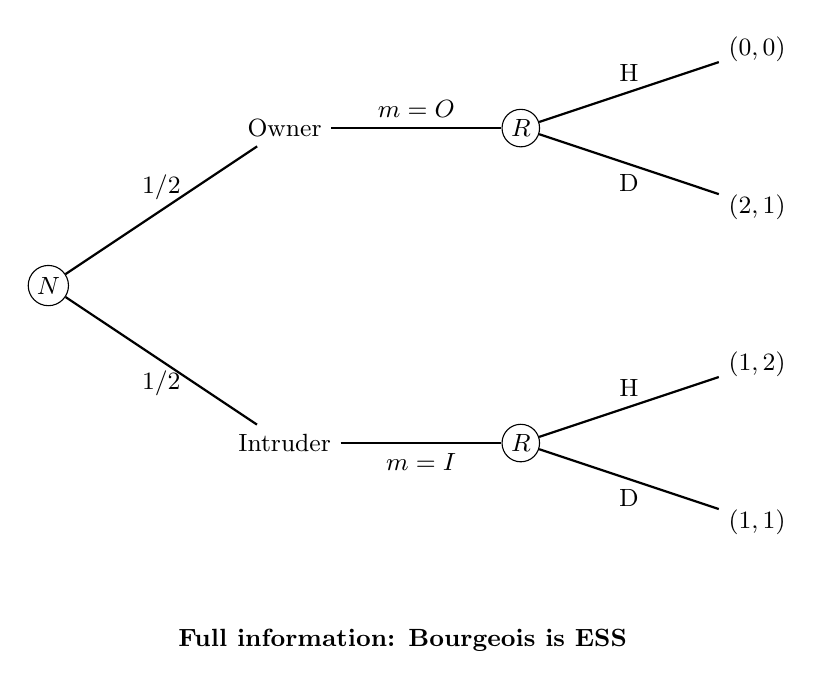
\begin{tikzpicture}[
    font=\small,
    decision/.style={circle,draw,inner sep=1.5pt},
    chance/.style={circle,draw,inner sep=1.5pt},
    line/.style={thick}
]

% Nature
\node[chance] (N) at (0,0) {$N$};

% Types
\node (O) at (3,2) {Owner};
\node (I) at (3,-2) {Intruder};

\draw[line] (N) -- node[above] {$1/2$} (O);
\draw[line] (N) -- node[below] {$1/2$} (I);

% Receiver nodes (один узел на тип)
\node[decision] (RO) at (6,2) {$R$};
\node[decision] (RI) at (6,-2) {$R$};

% Messages (однозначные)
\draw[line] (O) -- node[above] {$m=O$} (RO);
\draw[line] (I) -- node[below] {$m=I$} (RI);

% Payoffs (пример Bourgeois ESS)
\node (S1) at (9,3) {$(0,0)$};   % Owner H
\node (S2) at (9,1) {$(2,1)$};   % Owner D
\node (S3) at (9,-1) {$(1,2)$};  % Intruder H
\node (S4) at (9,-3) {$(1,1)$};  % Intruder D

\draw[line] (RO) -- node[above] {H} (S1);
\draw[line] (RO) -- node[below] {D} (S2);
\draw[line] (RI) -- node[above] {H} (S3);
\draw[line] (RI) -- node[below] {D} (S4);

\node at (4.5,-4.5) {\textbf{Full information: Bourgeois is ESS}};

\end{tikzpicture}

\end{document}
